\documentclass[twocolumn]{article}
\usepackage[utf8]{inputenc}
\usepackage{fullpage}
\usepackage{siunitx}
\usepackage{graphicx}

\title{Flexible, Changeable Potato Peeler}
\author{Lynne Diep}
\date{November 11, 2017}

\begin{document}

\maketitle

\section*{Abstract}
A tool to peel potato skin in one, circular movement around the whole potato rather than multiple top-down, uneven movements. The ``razor" of the peeler is made out of flexible plastic, which allows the peeler to form around the potato. Additionally, there are two size compressors for the peeler to fit potatoes of various sizes. There is a handle located at the bottom of the peeler to give the user a grip and stability to peel the potato. All materials used will be made out of durable plastic for the peeler to be dishwasher-safe and harmless in a home environment. The peeler will come pre-assembled, and the two size compressors will be packaged in the same box. Instructions and warnings will be provided in the packaging and online on the company's website. Note that the peeler is intended for potatoes only, and other objects used will not guarantee satisfactory results.
\section*{Prior Art}
Before adding the size compressors for the peeler, it was originally a flexible peeler. As seen in Figure 1, it was simple a peeler made out of the same durable plastic used in the current product. There are plastic bolts on each side of the peeler to secure the ``razor" in place. Around the razor is silicone molding to prevent unwanted objects near the ``razor", and for the possibility of the peeler slipping from the user's grasp. Once the user begins peeling the potato, the excess skin that has been peeled will exit the behind the ``razor". There is the option for the user to attach a container for the excess skin as seen in Figure 1.1. Once the container becomes full, it is up to the user to remove the container and empty it out and attach it back to the peeler for further use. However, due to the feedback received from multiple testers, the flexible peeler was more of a hassle than an efficient tool it strove to be. After more product design and modifications, the flexible peeler has become the product that it is currently.
\section*{Flexible, Changeable Potato Peeler}
The idea of the flexible, changeable potato peeler came from multiple complaints from the community of the tedious work of peeling vegetables; the vegetable with the most vocal opinion was the potato. Having a peeler solely for potatoes is a unique idea and useful due to the demand of potatoes in everyday cooking. Additionally potatoes are notorious difficult to peel due to the shape of it, so having a peeler dedicated to the potato will be welcomed from an abundance of audiences. The main issue with regular peelers was that the movement of peeling brought strain to users' wrists, and to those with arthritis extremely agreed with this point. So the objective of inventing a new and innovative peeler was to minimize the amount of wrist movement when peeling vegetables. The peeler had to be flexible in order to mold to the shape of the potato, since all potatoes come in different sizes and shapes. Safety was a concern when developing this idea as well, so the exchange of a plastic ``razor" instead of a metal one was logical. Additionally the use of a metal razor can lead for the peeler to rust and be unusable for future use. To find a plastic that is mold-able, bendable, sturdy, and can be found at a cost-efficient price was difficult. After researching for a plastic that can hold these qualities, polycarbonate plastic has proven to be the material used for the peeler. The plastic razor ensures the durability and reliability of the product.
\par
The design of the peeler comes from tradition peelers; the ``T" shaped peeler is the most common design for peelers due to its stability. If the handle of the peeler were placed elsewhere besides the middle, bottom on the peeler than it would be difficult to properly use the tool. The idea is not to produce the newest thing, but rather a modification of a stable tool in order to affect audiences of all backgrounds.
\par
Based on prior prototypes of the peeler, the current model still contains the idea of the two size compressors, durable plastic materials, and silicone molding.The feedback received from testers was that it was difficult to grasp the peeler in a comfortable and secure grip. With that in mind, the current model has a handle with a silicone strip on it to provide less friction. The length of the handle was based on the average fist size. Having a handle too long or too short would be awkward for the user and not giving them optimal leverage when peeling. When given this model to testers, they confirmed the handle definitely added more stability and comfort to the peeler. The handle also gives more leverage to the user and less accidents are to happened compared to the previous model where the user's hand is centimeters away from the ``razor".
\par
Regarding the two size compressors for the peeler, they are made out of the same durable plastic as the peeler. In the beginning of the design process, the compressors were able to tighten or loosen on a latch system. By pushing the latches down a few notches, the compressor would tighten. Pulling the latches apart would obviously loosen the compressor. However, this proved to be an issue when testers would peel their potatoes and the latches would come undone. The latch method was not a secure system and would become useless over time. So the current model has compressors that have knobs on the side to allow the user to open the width of it to allow easy assembly of the compressor onto the peeler. Depending on the size of the potato, the user is able to move the compressors to the appropriate size where the potato is firmly in between the two compressors and on the ``razor". Once everything is in place, turning the knobs right will tighten the compressors and will stay in place until the user turns the knobs to the left, which loosens the compressors. An accurate representation of the model with the compressors is presented in Figure 3. The use of the compressors are intuitive enough that those who participated in testing experiments needed little to no instructions on the proper handling of the tool.
\par
The reasoning why the two compressors are not permanently attached to the peeler is due to the unpredictable shape of the potato. Having the two compressors can get in the way when dealing with a large potato and affect the peeling process. Additionally having the two compressors present when not in use will make the product bulky and difficult to clean. Storage of the peeler was kept in mind as well; if the compressors were to remain on the peeler, then storage would be an issue due to the peculiar design and dimensions of it. The removal of the compressors allows the peeler to lie flat and can be stored in typical drawers found in a kitchen. The product is trying to make users' lives more efficient and not hinder them from using it due to inconvenience.
\par
When the potato is secured in place with the compressors, it is ready to be peeled. To peel the potato, the user should hold the potato vertically where the handle is either pointing to the left of right, depending on the dominant hand of the user. With the dominant hand on the handle, and the other holding the potato, the user will pull the handle in its direction its pointing at while applying slight pressure on the potato. Since the peeler is flexible and the potato is locked on to the peeler, the skin of the potato should be peeled in one fluid movement. The end result should be a perfectly skinned potato, where the peeled skin should be one long skin. If the user decides to not hold the peeler in this position, then the peeling of the potato will not go smoothly. The results of having perfectly skinned potato is not guaranteed, and the position of the wrist can cause strain and discomfort. Going back to prior art designs for the peeler, there was the idea of a skin container that can be attached to the back of the peeler. It was bulky and the process of emptying the container and attaching it back to peeler was unnecessary, and users will most likely avoid the skin container after the initial use. With consideration, the container will no longer be part of the current model as it adds no significant efficiency to the user and can get in the way of the peeling process.
\\
For better understanding of the invention reference used throughout the patent, the following is a description for each of the accompanying figures, in which:
\\
\indent{\textbf{Figure 1} - Frontal view of early prototype of peeler. Has the skin container attached.}
\\
\indent{\textbf{Figure 1.1} - Side view of early prototype with skin container attached.}
\\
\indent{\textbf{Figure 2} - Design of the two compressors.}
\\
\indent{\textbf{Figure 3} - Frontal view of early prototype of peeler with the two compressors attached.}
\\
\indent{\textbf{Figure 4} - Frontal view of current design of peeler with handle. Two compressors are presented and not attached to peeler.}
\par
The flexible, changeable potato peeler is efficient and easy to use. It is safer than most peelers being sold today, and its unique function of adapting to the size of the potato makes it different. When giving testers the current model of the peeler, they immediately felt and saw the differences and improvements on the tool compared to previous models. There was positive feedback on the handle of the peeler; testers stated that the handle definitely made the peeler more comfortable and easier to use. Users who complained about wrist aches on regular peelers stated that the flexibility and changeability of this peeler prevented wrist aches and allowed them to peel potatoes without hesitation. Furthermore, the cost to produce the peeler is cost-effective which allows the company to retail the peeler in affordable terms. By having an affordable, effective product on the market, there is a high chance of having a favorable outcome. Ultimately this take on the potato peeler is different and new. It adds more value than a regular peeler and produces satisfaction from customers. 
\section*{Claims}
\textbf{1.} The potato peeler is made out of durable, flexible plastic which allows the peeler to bend \ang{180} without breaking and loosing any of its ability. The length of the peeler is 4.5 inches in length and 2 inches in width. The outer area surrounding the ``razor" is silicone to prevent slipping from the potato and added protection to the user. There are plastic screws on the side of the peeler to hold the ``razor" in place. There is a plastic handle connected to the bottom of the peeler, and has a length of 4 inches and a width of 1 inch. On the side of the handle, there is a silicon layer wrapped around it. The silicon layer's purpose is to provide a better grip for the user and comfort. Two compressors are also apart of the peeler, but do not come attached to the peeler. The compressors are in the shape of a ring, with a diameter of 1.5 inches. There are knobs on the side of the compressors to tighten or loosen the rings and allow the user to attach them onto the peeler.
\\
\textbf{2.} The peeler as defined in claim \textbf{1} is design for potatoes in various sizes, and not for other objects.
\\
\textbf{3.} The potatoes defined in claim \textbf{2} can fit the dimensions of the peeler defined in claim \textbf{1}, and sizes over the dimensions are not guaranteed to fit the peeler.
\\
\textbf{4.} Using the peeler for other objects will not promise the same results if a potato was used for a peeler as defined in claim \textbf{2}.
\\
\textbf{5.} The handle defined in claim \textbf{1} is optimal for users with the appropriate hand size, and will the peeler will not work to its potential with users that have hand sizes over and under the dimensions.
\pagebreak
\section*{}
\section*{Drawings}
\begin{figure}[h]
    \centering
    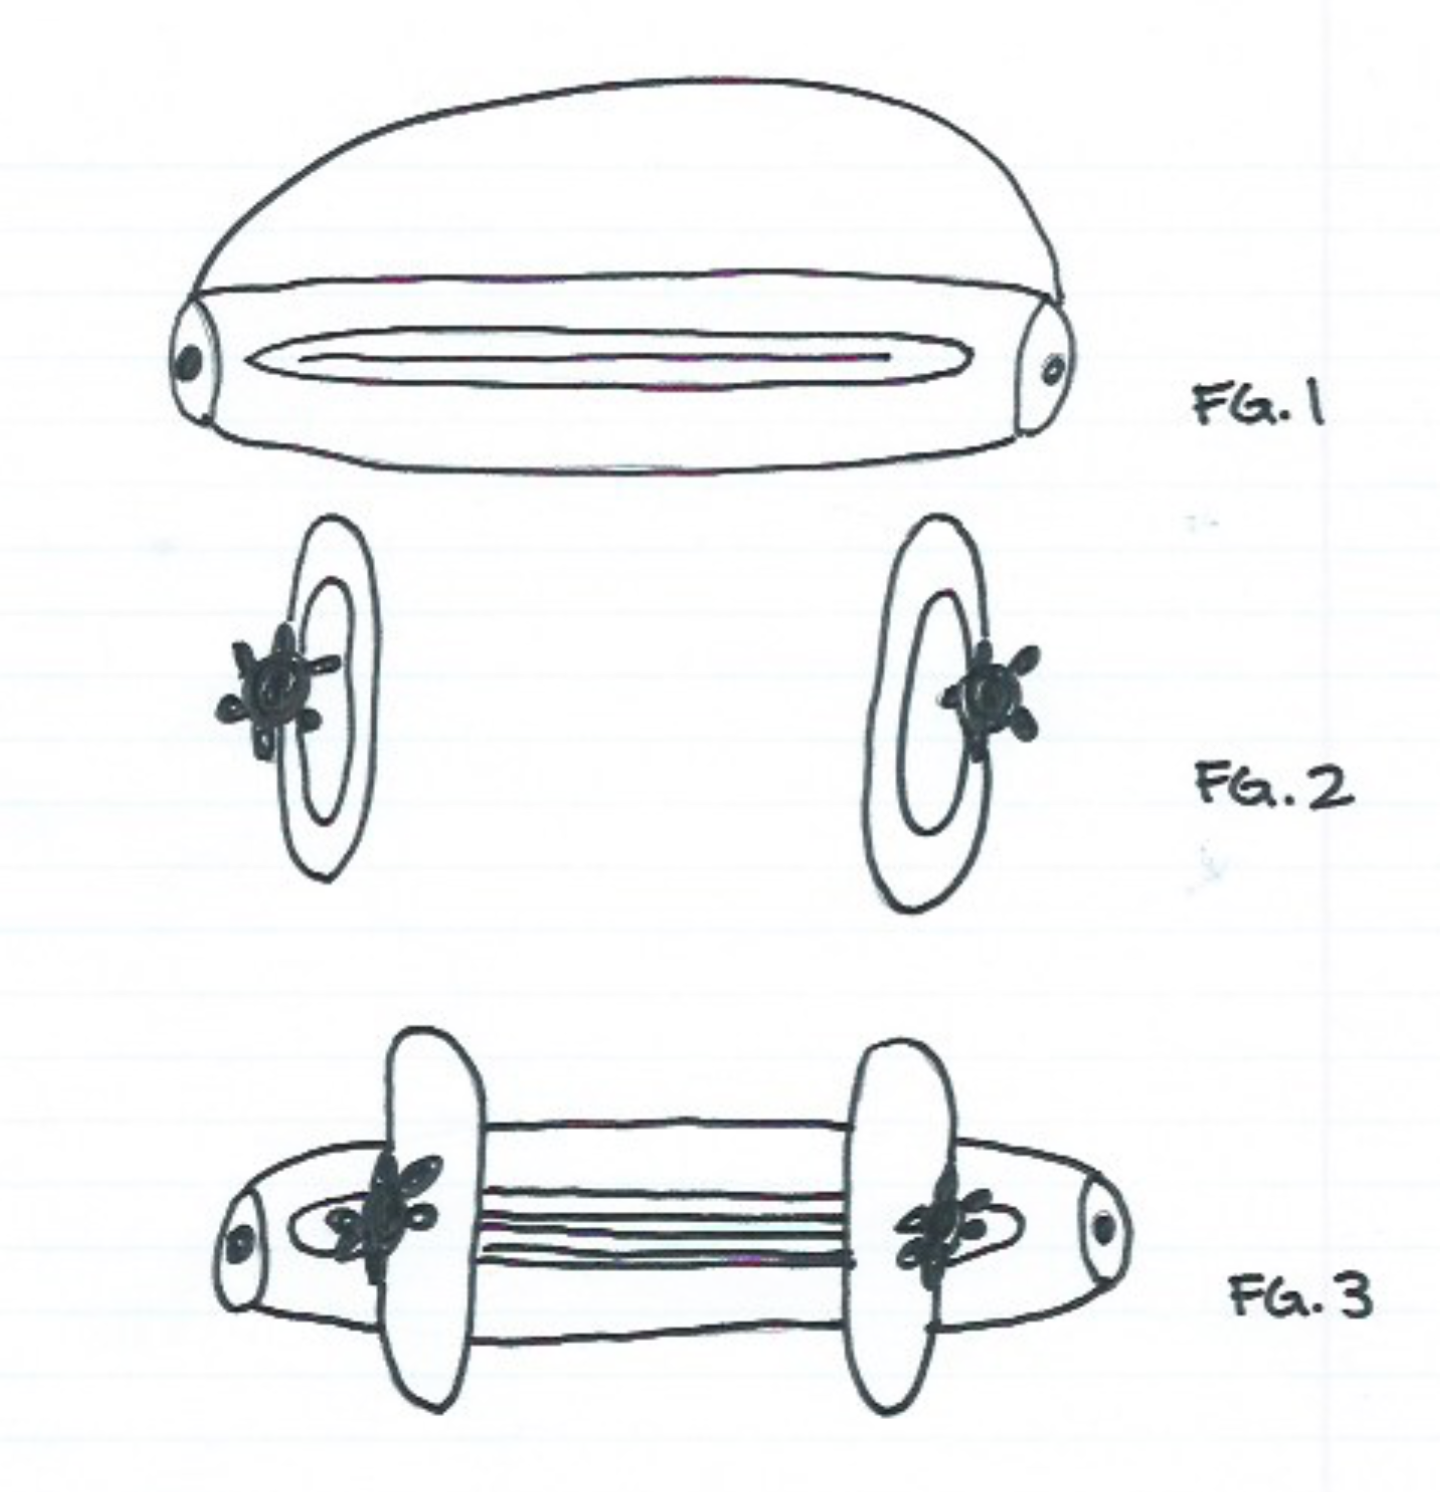
\includegraphics[width=400px]{potatopeeler}
\end{figure}
\newpage
\section*{}
\newpage
\begin{figure}[h]
    \centering
    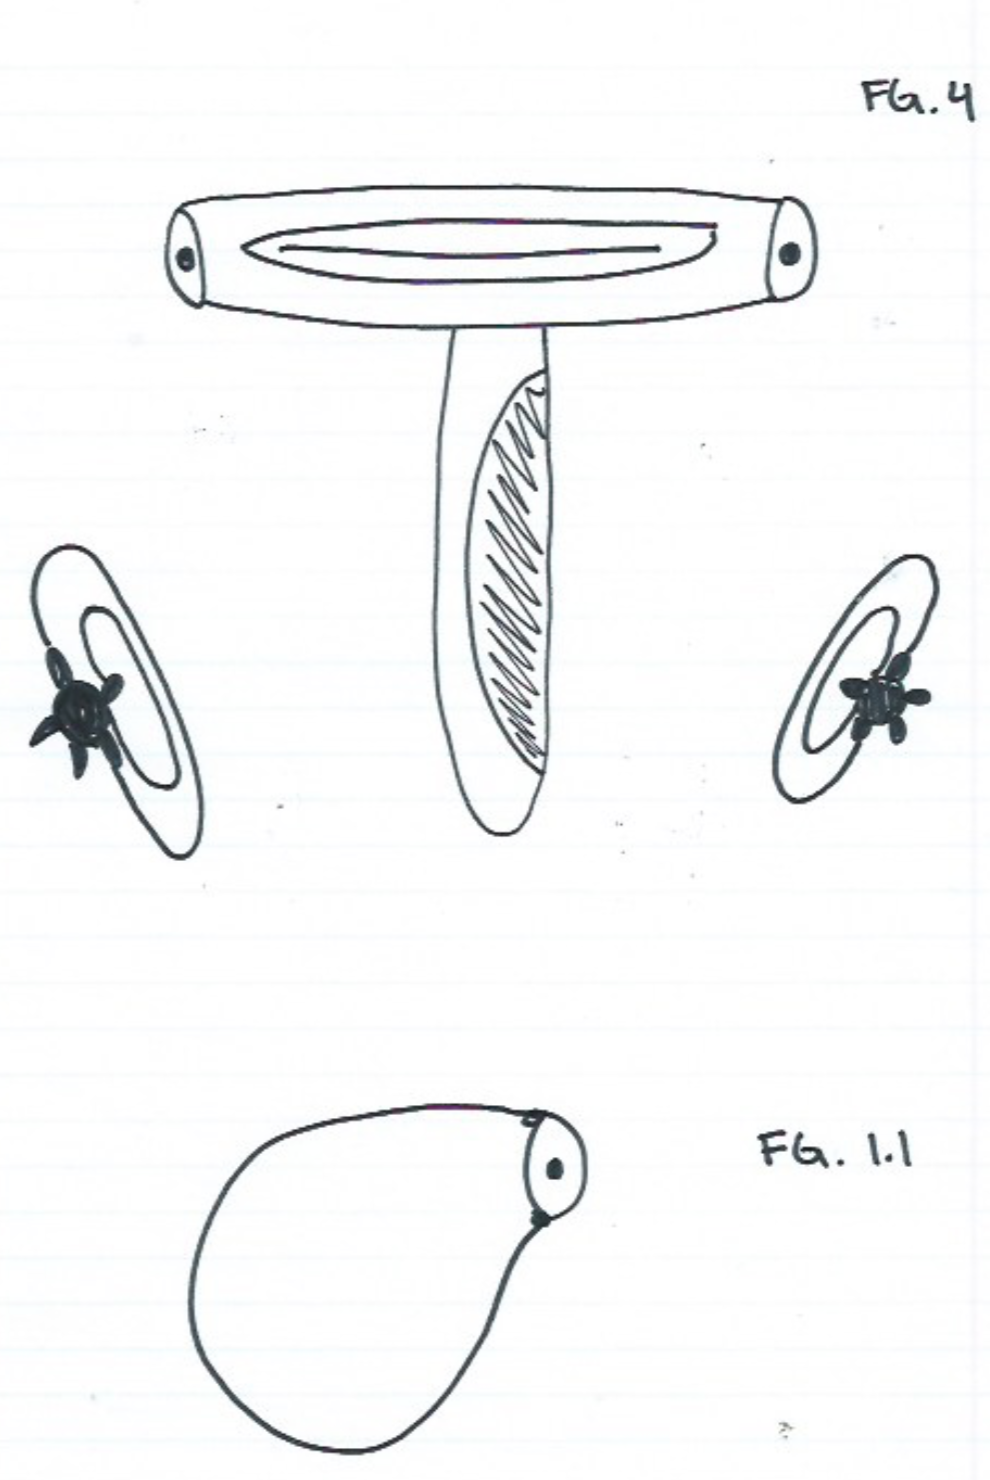
\includegraphics[width=400px]{potatopeeler2}
\end{figure}
\end{document}
